\newpage
\section{人体几何模型的应用}
\subsection{问题描述}
在上一部分中,我们已经从图片中得到人体的三维关节点的坐标,但是在实际应用中,简单的骨架表示不够具有表现力,因此最新的论文里的做法是使用一个预先生成好的参数化的人体几何模型,通过优化算法,或者直接通过网络估计,得到该模型的参数。在我们的问题中,希望通过输入一个人体的骨架的三维坐标,输出该参数化模型的参数。由于骨架坐标无法完全确定该模型的参数,因此我们需要引入一些额外的约束,来完成该求解过程。

\subsection{模型介绍}
SMPL模型是一个高效的线性人体模型,模型总共定义了\(N = 6890\)个顶点,作为人体的模板\(\bar{\bm{T}}\)。为了使该模型能够描述不同的人体姿态,该模型定义了人体的24个关节,每个关节具有三个旋转的自由度(包括整个身体的旋转),再加上身体的平移的三个自由度,该模型使用了\(3\times 24 + 3 = 75\)个位姿参数\(\theta\)来描述人体的姿态。为了能够描述不同人体的形状的差异,模型使用了形状参数\(\beta\)来对人体模板的点进行非刚性变形。也就是说,人体模板首先会根据形状参数和姿态参数进行变形:
\begin{equation}
    T(\beta, \theta) = \bar{\bm{T}} + B_S(\beta) + B_P(\theta)
\end{equation}
这里的\(B_S(\beta)\)是一个形状混合函数,他将形状参数\(\beta \in \mathbb{R}^{|\beta|}\)映射到人的模型的顶点所在的空间内,即\(B_S(\beta):\mathbb{R}^{|\beta|} \mapsto \mathbb{R}^{3N}\)。这里的\(B_P(\beta)\)是一个依赖于姿势的形状混合函数,他将姿势参数\(\theta \in \mathbb{R}^{|\theta|}\)同样映射到人的模型的顶点所在的空间内,即\(B_P(\beta):\mathbb{R}^{|\theta|} \mapsto \mathbb{R}^{3N}\),这一项考虑的是人体在进行不同的动作的时候,对身体的造成的形变。这两项形状混合函数都是直接将点的坐标加到人体的静止姿态下,也就是说先对人体的静止姿态进行变形,完成对形状的改变。在这之后,再对人体模型上的所有点进行混合蒙皮操作(blend skinning),将非关键点的位置进行旋转平移,得到经过姿势变换后的人体模型上的点的位置。

\textbf{混合蒙皮(Blend skinning):}这一步的目的是为了根据输入的姿态参数\(theta\)将人体的网格模型进行变形。人体的姿态参数的定义是,对于每个关节,使用轴角(axis-angle)来表示他的旋转。由于每一个旋转矩阵只有三个自由度,所以一般的表示方法都是使用参数化的表示。常用的参数化的方法是使用欧拉角,但是欧拉角会带来万向锁的问题,因为欧拉角表示并没有覆盖旋转矩阵空间内的所有区域。并且,欧拉角使用角度来进行表示,这样在进行优化的时候其值的范围是有周期性的,不连续,使得优化过程不自然,因此选择了使用轴角表示。

对于我们的骨架模型,有\(K=23\)个关节表示旋转,加上人整体的旋转,姿势参数即为\(\theta = [\omega_0^T, \omega_1^T, \ldots, \omega_K^T]\),其中的每一个\(\omega\)是一个三维的向量,\(\omega\)的模长\(||\omega||\)表示旋转的角度,\(\frac{\omega}{||\omega||}\)表示旋转的方向的单位向量。为了在计算的时候表示旋转,通常会需要先转换成旋转矩阵。旋转向量转化成旋转矩阵的方法是通过罗德里格斯公式(Rodrigues formula):
\begin{equation}
    \exp \left(  \omega  _ { j } \right) = \mathcal { I } + \widehat { \overline { \omega }} _ { j } \sin \left( \left\|  \omega  _ { j } \right\| \right) + \widehat { \overline { \omega } } _ { j } ^ { 2 } \cos \left( \left\| \omega_ { j } \right\| \right)
\end{equation}
其中\(\overline { \omega } = \frac{\omega}{||\omega||}\)表示旋转轴的单位向量,\(\widehat { \overline { \omega }}\)表示关于三维向量\(\overline{\omega}\)的反对称矩阵,即对于向量\(\mathbf{K} = [k_x, k_y, k_z]^T\),其计算公式为
\begin{equation}
\widehat{\mathbf { K }} = \left[ \begin{array} { c c c } { 0 } & { - k _ { z } } & { k _ { y } } \\ { k _ { z } } & { 0 } & { - k _ { x } } \\ { - k _ { y } } & { k _ { x } } & { 0 } \end{array} \right]
\end{equation}
\(\mathcal { I }\)表示\(3\times 3\)的单位矩阵。那么通过这一步计算,我们即将所有的\(K \times 3\)的旋转向量转换成了\(K\times 3 \times 3\)的旋转矩阵。由于在进行点的坐标计算的时候,一般都使用齐次坐标来表示点的位置,因此我们需要将旋转矩阵扩充为\(4\times 4\)的齐次变换矩阵。也即是说对于每个关节,都有一个局部的齐次变换矩阵,写为
\begin{equation}
\left[ \begin{array} { c | c } { \exp \left( \vec { \omega } _ { j } \right) } & { \mathbf { j } _ { j } } \\ \hline \overrightarrow { 0 } & { 1 } \end{array} \right]
\end{equation}
计算该关节相对于全局坐标系的齐次变换矩阵时,即需要根据骨架连接的顺序,依次将各个关节的局部变换矩阵相乘,即可得到该关节的全局变换矩阵,即
\begin{equation}
    G _ { k } ( \vec { \theta } , \mathbf { J } ) = \prod _ { j \in A ( k ) } \left[ \begin{array} { c | c } { \exp \left( \vec { \omega } _ { j } \right) } & { \mathbf { j } _ { j } } \\ \hline \overrightarrow { 0 } & { 1 } \end{array} \right]
\end{equation}
其中,\(A(k)\)表示对于关节\(k\),其所有父节点的按连接顺序排列的有序集合。\comment{插个图片,举个例子}。该式子表示,对于关节\(k\),其全局变换矩阵的计算为其父节点的全局变换矩阵的依次矩阵相乘。\(\mathbf{j}_j\)表示关节\(j\)的相对于其父节点的位移,其长度即为该段骨长。在计算时,考虑到在初始状态时模型的点的位置应该不发生改变,因此需要构造一个矩阵去掉初始状态的影响。计算公式为
\begin{equation}
    G _ { k } ^ { \prime } ( \vec { \theta } , \mathbf { J } ) = G _ { k } ( \vec { \theta } , \mathbf { J } ) G _ { k } \left( \vec { \theta } ^ { * } , \mathbf { J } \right) ^ { - 1 }
\end{equation}
那么通过加权融合,作用到所有点上,得到变形过后的点的位置,计算公式为
\begin{equation}
    \overline { \mathbf { t } } _ { i } ^ { \prime } = \sum _ { k = 1 } ^ { K } w _ { k , i } G _ { k } ^ { \prime } ( \vec { \theta } , \mathbf { J } ) \overline { \mathbf { t } } _ { i }
\end{equation}
该式子表示对于第\(i\)个点,其在变形后的初始状态的齐次坐标为\(\overline{\mathbf{t}}\),这个点关于身体的第\(k\)个部分的权重为\(w_{k,i}\)。\(w_{k,i}\)是混合权重矩阵\(\mathcal{W}\)的元素,在这里,模型假设身体上的每一个顶点至多只与4个关节有关,也就是说至多有四个关节的旋转矩阵会影响到一个顶点的旋转,在程序实现的时候,\(\mathcal{W}\)是一个稀疏矩阵,这样也可以提高计算效率。模型的计算过程如图\ref{fig:smpl}所示。
\begin{figure}[htbp]
    \centering
    \includegraphics[width=\linewidth]{figure/smpl/smpl}
    \caption{\label{fig:smpl} SMPL模型示意图。(a)模型模板网格,其中的颜色表示混合权重,关节点用白色圆点标出;(b)考虑形状参数的模板变形;(c)考虑姿态参数的模板变形;(c)通过姿态参数使所有的点进行变形}
\end{figure}
综合以上过程,模板上的的点\(\overline { \mathbf { t } } _ { i }\)的形变计算过程可以写为
\begin{equation}
    \overline { \mathbf { t } } _ { i } ^ { \prime } = \sum _ { k = 1 } ^ { K } w _ { k , i } G _ { k } ^ { \prime } ( \vec { \theta } , J ( \vec { \beta } ) ) \left( \overline { \mathbf { t } } _ { i } + \mathbf { b } _ { S , i } ( \vec { \beta } ) + \mathbf { b } _ { P , i } ( \vec { \theta } ) \right)
\end{equation}
其中的\(\mathbf{b}_{S,i}(\beta), \mathbf{b}_{P,i}(\theta)\) 分别表达对于点\(\overline { \mathbf { t } } _ { i }\),根据形状参数混合的偏移量与姿态混合的偏移量。那么就是说,网格的所有点的位置即是一个关于形状和姿态参数的函数,我们通过这个函数就可以使用低维的参数来表达高维的点的坐标数据,这也使得对这个问题进行的优化提供了可能。如图\ref{fig:smplsample},图中即为根据不同的形状和姿势参数计算得到的不通形状和姿势的人体模型,可以看出该模型表现能力较强,能够适应大范围的不同样式的人体的姿态,同时还能对不通高矮胖瘦的人体提供一个较好的表达。

\begin{figure}[htbp]
    \centering
    \includegraphics[width=0.8\linewidth]{figure/proposal/smpl}
    \caption{\label{fig:smplsample} SMPL模型示例}
\end{figure}

\subsection{模型拟合}
要将人体模型拟合到我们的骨架上,由于模型参数有\(3\times 23 + 3\)个姿态参数和10个形状参数,而我们的输入只有\(N \times 3\)个关节点的坐标,如果使用AlphaPose进行关节点估计,那么就只有\(17 \times 3\)个关节的三维位置,因此无法直接通过求解方程的方式将参数求解出来,并且该方程也是一个高度非线性的方程,直接求解比较困难。同时,该模型表达的每个关节具有3个自由度,而使用骨架来表示的人体的自由度并没有三个,每个骨架上的关节至多只能表示两个方向的旋转。因此在求解该问题时,我们仍然是将其转化为一个优化问题来进行求解,通过增加先验条件作为优化问题的损失函数,来求解这个问题。以下依次介绍考虑该问题时的优化项。

\textbf{三维关节误差:}这一项的含义是我们希望拟合得到的模型的关节点的三维坐标与我们在前一步通过多个视角的二维坐标恢复出来的三维坐标尽量一致,也就是说通过该项使得三维模型尽量贴合恢复出的三维关节坐标。用\(X_{est}\)表示估计得到的三维关节坐标,那么关于关节的损失函数即写为
\begin{equation}
    L_{J3d}(\beta, \theta; X_{est}) = \sum_{\text{关节}i}w_i\rho||J(\theta, \beta) - X_{est}||
\end{equation}
其中\(J(\theta, \beta)\)表示SMPL人体模型计算得到的关节坐标,\(w_i\)表示关节\(i\)的权重,加入该权重是因为在前一步的估计中,三维坐标是具有不确定性的,我们希望通过这一项使得准确估计出来的关节权重更高,而置信度低的关节权重低一点,该权重是由各个视角下的二维关节点的检测的置信度求和得到。\(\rho\)表示鲁棒的核函数,这里使用的是Huber核函数,该函数在函数值较大时可以将其梯度变为0,一般在优化问题中通常用该函数来去掉离群值(outlier)的影响,使得求解更鲁棒。

\textbf{二维关节误差:}虽然之前恢复出来的三维关节坐标已经将之前的二维关节的值包含了,但是将三维关节投影到各个相机上可以使得求解的结果更稳定,我们仍然可以充分利用之前的二维关节检测结果来继续进行优化。与之前的写法类似
\begin{equation}
    L_{2d} = \sum^I_{i=1} \sum_{n=1}^N w_{in}||Z_i^{-1}K_i(R_iJ(\theta, \beta)_n + T_i) - \hat x_{in}||_2
\end{equation}

\textbf{反关节误差:}对于人体来说,部分关节是只能像一个方向旋转的,即人的左手手腕与右手手腕,以及人的左脚膝盖与右脚膝盖,这四个关节都只能向一个方向弯曲,那么我们增加这一项去惩罚人的不自然的弯曲:
\begin{equation}
    L_{un}(\theta) = \sum_i \exp(\c_i\theta_i)
\end{equation}
这里的\(i\)即对相应的膝盖与手腕的旋转参数进行求和,\(c_i\)控制正确的旋转方向。例如,膝关节向后弯曲是正常的弯曲,此时\(\theta>0\),那么他对应的系数\(c_i = -1\),即使得当\(\theta_i>0\)时,该项的值较小;而如果此时膝关节向前弯曲,那么该项的值就会较大。通过指数函数,可以在这几个关节进行错误的方向的旋转的时候损失增长较快,而如果是正常的弯曲方向的时候,那么该项的值就接近于0,不会提供较大的梯度。

\textbf{时序误差:}我们都知道,人体是具有骨架结构的,也就是说人的运动状态一定是连续的,人的关节坐标无法突变,因此,为了增加结果的鲁棒性,以及重建的人的运动的平滑性,我们通过增加时序误差来对求解结果进行优化。时序误差的定义为

\begin{align} 
    L_ { T } ( \beta , \theta ) = \sum _ { t = 2 } ^ { T } \sum _ { i = 1 } ^ { J } \lambda _ { 1 } \left( \mathbf { X } _ { i } ^ { t } - \mathbf { X } _ { i } ^ { t - 1 } \right) + \lambda _ { 2 }\left( \mathbf { x } _ { i } ^ { t } - \mathbf { x } _ { i } ^ { t - 1 } \right)
\end{align}

式中,$X$ 表示人体的关节点的三维坐标,$X_i^t$ 表示在第$t$时刻人体的第$i$个关节的三维空间位置。同样,我们可以将人体的三维关节点坐标投影到像素坐标系中,得到人体的二维关节点位置,我们希望在像素坐标系中,人体的运动同样也是平滑的,因此式中$x_{ic}^t$ 表示在$t$时刻人体的第$i$个关节在第$c$个相机的视角下的二维关节点位置。
 
\textbf{先验姿势:}对于人体来说,我们知道有许多姿态都是不合理的,也就是说,我们可以对人体的姿态分布有一个先验的知识。而这种先验知识我们可以从大规模的基于标记点的运动捕捉系统中得到。通过基于标记点的运动捕捉系统,我们可以得到许多不同的人的日常动作,从这些动作中我们可以预先学习得到人体的动作分布。一般的动作捕捉数据集中包含了大量的人体动作,为了简化模型参数,一般的做法是使用一个混合高斯模型去拟合人体的动作数据。在判断一个姿态是否属于正常的人体姿态时,通常对混合高斯模型构造一个负对数似然函数,以该函数作为损失函数,然后最小化这个函数的值。即%\unsure{}{这里写得内容不够}
$$
    L_ { J } ( \theta ) = - \log \left( \sum _ { i } g _ { i } \mathcal { N } \left( \theta ^ { t } ; \mu _ { i } , \Sigma _ { i } \right) \right)
$$
式中,$\mu_i, \Sigma_i$ 分别表示第$i$个高斯分布的均值和协方差,$g_i$ 表示第$i$个高斯分布的权重。通过这种方式,可以表达分布差异较大的人体姿态,并且这些姿态都是属于人体可能存在的姿态。我们使用了Bogo\cite{bogo2016keep}等人提供的人体姿势的混合高斯分布参数先验,作为损失函数里面的参数。

\subsection{优化过程}
SMPL的官方提供的模型使用chumpy实现,chumpy是基于Python的自动微分库,但是该库过于陈旧,并且只能使用CPU进行计算,无法使用GPU提高计算速度,而在SMPL模型的计算过程中,会有大量的矩阵乘法的计算,而这种计算在CPU上的计算速度是远低于GPU的。在优化的过程中,单步计算的速度对整个优化过程的计算时间影响巨大,因此为了提高优化时间,我们使用PyTorch\cite{pytorch}对该模型进行了重新实现。
PyTorch是基于Python的GPU张量计算库,该库使用C++实现底层算法,并提供了Python接口,可以较为方便的调用。同时,PyTorch还是一个广泛使用的深度学习框架,它的优势在于动态建立计算图,较为灵活。同时,对于优化问题来说,它还提供了方便的自动求导技术。

求解时我们使用PyTorch的梯度下降法进行求解,求解算法使用BFGS,对于第一帧我们从初始状态作为初始值进行优化,对于之后的每一帧,我们使用前一帧的求解参数作为初始值进行优化。第一帧的优化耗时10s左右,之后每一帧的优化耗时在2s以下。

% \comment{抄一下LBFGS}
% \textbf{拟牛顿法:}拟牛顿法是对牛顿法进行近似的方法,适用于无法求解海森矩阵或者海森矩阵较难求解的情况。主要的思想是根据损失函数的梯度的差分,能够构造出损失函数的海森矩阵的某种近似,再根据牛顿法的方程得到更新的方向,最后再通过线搜索方法完成迭代。与之前的方法类似,在\(x_{n_1}\)处对损失函数进行泰勒展开,得到
% \begin{equation}
%     E(x) \approx E(x_{n+1}) + (x - x_{n+1}) ^T \nabla E(x_{n+1}) + \frac{1}{2}(x-x_{n+1})^T (\nabla^2 E(x_{n+1}))(x-x_{n+1})
% \end{equation}
% 等式两段对\(x\)求梯度,可以得到
% \begin{equation}
%     \nabla E(x) \approx \nabla E(x_{n+1}) +\nabla^2 E(x_{n+1})(x-x_{n+1})    
% \end{equation}
% 将\(x = x_n\)代入上式,可以得到
% \begin{equation}
%     \nabla E(x_n) \approx \nabla E(x_{n+1}) +\nabla^2 E(x_{n+1})(x_n-x_{n+1})    
% \end{equation}
% 整理之后得到
% \begin{equation}
%     \nabla^2 E(x_{n+1})(x_{n+1} - x_n)  = \nabla E(x_{n+1}) - \nabla E(x_n)
% \end{equation}
% 为了简化式子,记
% \begin{equation}
%     s_k=x_{k+1}-x_k, y_k=\nabla f_{k+1}-\nabla f_k
% \end{equation}
% 将海森矩阵用其近似矩阵\(B_{n+1}\)来代替,那么则有
% \begin{equation}
%     B_{n+1}s_k = y_k
% \end{equation}


% \textbf{BFGS算法:}BFGS算法是Broyden, Fletcher, Goldfarb和Shanno四个发明者的名字的首字母命名的,目前该算法是求解无约束非线性问题的最常用方法之一。他的主要思想是不断地去逼近海森矩阵,其更新方式为
% \begin{equation}
%     H_{k+1} = H_k + \Delta H_k, k=0,1,2,\ldots
% \end{equation}
% 其初值通常选为单位矩阵。从公式\ref{eq:newton}可以看出来,当海森矩阵为单位矩阵时,该更新方向就是其梯度方向,那么这个时候算法就退化为梯度下降方法了

\subsection{模型应用}
最后,我们将上述优化过程应用到我们的数据上,如图\ref{fig:smpljoint}所示。图中为之前选择的三个不同人物的对应的帧,我们可视化的时候选择了两个不同的视角,体现出求解算法的适应性,说明我们的求解过程能够较好地完成使用人体模型来表示人体关节点的过程。
\begin{figure}[htbp]
    \centering
    \includegraphics[height=0.325\linewidth]{figure/result/images/feng2} \hfill
    \includegraphics[height=0.325\linewidth]{figure/result/smpl/feng1} \hfill
    \includegraphics[height=0.325\linewidth]{figure/result/smpl/feng2} \hfill
    \includegraphics[height=0.325\linewidth]{figure/result/images/shuai2} \hfill
    \includegraphics[height=0.325\linewidth]{figure/result/smpl/shuai1} \hfill
    \includegraphics[height=0.325\linewidth]{figure/result/smpl/shuai2} \hfill
    \includegraphics[height=0.325\linewidth]{figure/result/images/ke2} \hfill
    \includegraphics[height=0.325\linewidth]{figure/result/smpl/ke1} \hfill
    \includegraphics[height=0.325\linewidth]{figure/result/smpl/ke2} 
    \caption{三维模型重建结果,左列为原始图片,中间列为当前视角下的三维模型,第三列为另一视角的三维模型\label{fig:smpljoint}}
\end{figure}